\newcommand{\UTxOEpState}{\type{UTxOEpState}}
\newcommand{\Acnt}{\type{Acnt}}
\newcommand{\RewardEnv}{\type{RewardEnv}}
\newcommand{\RewardState}{\type{RewardState}}
\newcommand{\PlReapState}{\type{PlReapState}}
\newcommand{\PlReapEnv}{\type{PlReapEnv}}
\newcommand{\NewPParamEnv}{\type{NewPParamEnv}}
\newcommand{\Snapshots}{\type{Snapshots}}
\newcommand{\SnapshotEnv}{\type{SnapshotEnv}}
\newcommand{\SnapshotState}{\type{SnapshotState}}
\newcommand{\NewPParamState}{\type{NewPParamState}}
\newcommand{\EpochEnv}{\type{EpochEnv}}
\newcommand{\EpochState}{\type{EpochState}}
\newcommand{\BlocksMade}{\type{BlocksMade}}
\newcommand{\Stake}{\type{Stake}}
\newcommand{\PooledStake}{\type{PooledStake}}
\newcommand{\Avgs}{\type{Avgs}}

\newcommand{\obligation}[4]{\fun{obligation}~ \var{#1}~ \var{#2}~ \var{#3}~ \var{#4}}
\newcommand{\reward}[7]{\fun{reward}
  ~ \var{#1}~ \var{#2}~ \var{#3}~ \var{#4}~ \var{#5}~ \var{#6}~ \var{#7}}
\newcommand{\rewardOnePool}[9]{\fun{rewardOnePool}
  ~\var{#1}~\var{#2}~\var{#3}~\var{#4}~\var{#5}~\var{#6}~\var{#7}~\var{#8}~\var{#9}}
\newcommand{\isActive}[4]{\fun{isActive}~ \var{#1}~ \var{#2}~ \var{#3}~ \var{#4}}
\newcommand{\activeStake}[5]{\fun{activeStake}~ \var{#1}~ \var{#2}~ \var{#3}~ \var{#4}~ \var{#5}}
\newcommand{\poolRefunds}[3]{\fun{poolRefunds}~ \var{#1}~ \var{#2}~ \var{#3}}
\newcommand{\poolStake}[4]{\fun{poolStake}~ \var{#1}~ \var{#2}~ \var{#3}~ \var{#4}}
\newcommand{\poolDistr}[3]{\fun{poolDistr}~ \var{#1}~ \var{#2}~ \var{#3}}
\newcommand{\lReward}[4]{\fun{r_{leader}}~ \var{#1}~ \var{#2}~ \var{#3}~ {#4}}
\newcommand{\mReward}[4]{\fun{r_{member}}~ \var{#1}~ \var{#2}~ \var{#3}~ {#4}}
\newcommand{\poolReward}[6]{\fun{poolReward}~\var{#1}~\var{#2}~\var{#3}~\var{#4}~\var{#5}~\var{#6}}
\newcommand{\movingAvg}[5]{\fun{movingAvg}~ \var{#1}~ \var{#2}~ \var{#3}~ \var{#4}~ \var{#5}}
\newcommand{\updateAvgs}[4]{\fun{updateAvgs}~ \var{#1}~ \var{#2}~ \var{#3}~ \var{#4}}

This chapter introduces two main transition systems.
Neither transition is triggered by a transaction, and in fact have no signal.

The first one, defined in Section~\ref{sec:total-epoch},
involves calculations that occur at the epoch boundary.
This includes taking stake distribution snapshots
(Sections \ref{sec:stake-dist} and \ref{sec:snapshots}),
retiring stake pools (Section \ref{sec:pool-reap}),
and performing protocol updates (Section \ref{sec:pparam-update}).
The second transition, defined in Sections ~\ref{sec:reward-dist} and ~\ref{sec:reward-trans},
distributes the leader election rewards.

\subsection{Overview of the Reward Calculation}
\label{sec:reward-overview}

The rewards for a given epoch $e_i$ involve the two epochs surrounding it.
In particular, the stake distribution will come from the previous epoch,
and the rewards will be calculated in the following epoch.
More concretely:
\begin{enumerate}[(A)]%for small alpha-characters within brackets.
  \item A stake distribution snapshot is taken at the begining of epoch $e_{i-1}$.
  \item The randomness for leader election is fixed during epoch $e_{i-1}$
  \item Epoch $e_{i}$ begins.
  \item Epoch $e_{i}$ ends.
    A snapshot is taken of the stake pool performance during epoch $e_{i}$.
    A snapshot is also taken of the fee pot and the decayed deposit values.
  \item The snapshots from (D) are stable and the reward calculation can begin.
  \item Rewards are given out.
\end{enumerate}

\usetikzlibrary{decorations.pathreplacing}
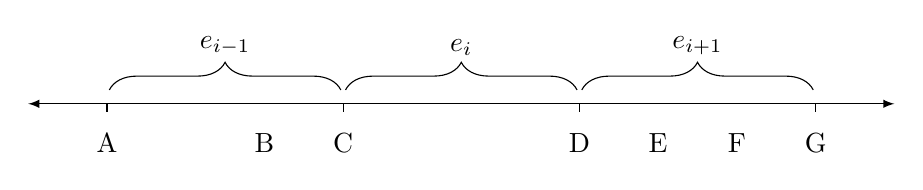
\begin{tikzpicture}
% axis
\draw[latex-latex] (0,0) -- (11,0) ;

% epoch braces
\draw [decorate,decoration={brace,amplitude=10pt} ,yshift=5pt] (1.03,0) -- (3.97,0)
  node [midway, above, yshift=9pt]{$e_{i-1}$};
\draw [decorate,decoration={brace,amplitude=10pt} ,yshift=5pt] (4.03,0) -- (6.97,0)
  node [midway, above, yshift=9pt]{$e_{i}$};
\draw [decorate,decoration={brace,amplitude=10pt} ,yshift=5pt] (7.03,0) -- (9.97,0)
  node [midway, above, yshift=9pt]{$e_{i+1}$};

% epoch boundaries
\foreach \x in  {1,4,7,10}
  \draw[shift={(\x,0)}] (0pt,0pt) -- (0pt,-3pt);

\node at (1,-0.5) {A};
\node at (3,-0.5) {B};
\node at (4,-0.5) {C};
\node at (7,-0.5) {D};
\node at (8,-0.5) {E};
\node at (9,-0.5) {F};
\node at (10,-0.5) {G};

\end{tikzpicture}

We must therefore store the last three stake distributions.
The mnemonic ``mark, set, go'' will be used to keep
track of the snapshots, where the label ``mark'' refers to the most recent snapshot,
and ``go'' refers to the snapshot that is ready to be used in the reward calculation.
In the above diagram, the snapshot taken at (A) is labeled``mark'' during epoch $e_{i-1}$,
``set'' during epoch $e_i$, and ``go'' during epoch $e_{i+1}$. At (G) the snapshot
taken at (A) is no longer needed and will be discarded.

The two main transition systems in this section are:
\begin{itemize}
  \item The transition system named $\mathsf{EPOCH}$, which is defined in
    Section~\ref{sec:total-epoch}, covering what happens at the epoch boundary,
    such as at (A), (C), (D), and (G).
  \item The transition named $\mathsf{REWARD}$, which is defined in Section~\ref{sec:reward-trans},
    covering the reward calculation which happens between (E) and (F).
\end{itemize}

\subsection{Helper Functions}
\label{sec:stake-dist}

Figure~\ref{fig:funcs:epoch-helper} defines three helper functions needed
throughout the rest of the section.

\begin{itemize}
  \item The function $\fun{obligation}$ calculates the the minimal amount of coin needed to
    pay out all deposit refunds, as of the current slot.
  \item The function $\fun{poolRefunds}$ is used to calculate the total refunds
    that must be distributed for stake pools scheduled to retire.
    Note that this calculation takes a slot number corresponding to the epoch boundary slot
    when the calculation is performed.  The returned map maps pool operator hashkeys to the
    refunds, which will ultimately be returned to the registered reward account.
  \item The function $\fun{updateAvgs}$ calculates the new performance moving averages.
\end{itemize}


%%
%% Figure - Helper Functions for Epoch Rules
%%
\begin{figure}[htb]
  \emph{Total possible refunds}
  \begin{align*}
      & \fun{obligation} \in \PParams \to \StakeKeys \to \StakePools \to \Slot \to \Coin \\
      & \obligation{pp}{stkeys}{stpools}{cslot} =\\
      & \sum\limits_{(\_ \mapsto s) \in \var{stkeys}}
        \refund{d_{\mathsf{val}}}{d_{\min}}{\lambda_d}{(\slotminus{cslot}{s})}
        + \sum\limits_{(\_ \mapsto s) \in \var{stpools}}
        \refund{p_{\mathsf{val}}}{p_{\min}}{\lambda_p}{(\slotminus{cslot}{s})} \\
      &
      \begin{array}{lr@{~=~}l}
        \where
          & \dval,~d_{\min},~\lambda_d
          & \fun{keyDeposit}~\var{pp},~\fun{keyMinRefund}~\var{pp},~\fun{keyDecayRate}~\var{pp}
          \\
          & p_{\mathsf{val}},~p_{\min},~\lambda_p
          & \fun{poolDeposit}~\var{pp},~\fun{poolMinRefund}~\var{pp},~\fun{poolDecayRate}~\var{pp}
      \end{array}\\
  \end{align*}
  \emph{Pool refunds}
  \begin{align*}
      & \fun{poolRefunds} \in \PParams \to (\HashKey_{pool} \mapsto \Epoch) \to \Slot \to
      (\HashKey_{pool} \mapsto \Coin) \\
      & \poolRefunds{pp}{retiring}{cslot} = \left\{
        \var{hk}\mapsto
          \refund{p_{\mathsf{val}}}{p_{\min}}{\lambda}{(\slotminus{cslot}{(\fun{slot}~e)})}
          \mid
          \var{hk}\mapsto e\in\var{retiring}
        \right\}\\
      & \where p_{\mathsf{val}},~p_{\min},~\lambda_p =
          \fun{poolDeposit}~\var{pp},~\fun{poolMinRefund}~\var{pp},~\fun{poolDecayRate}~\var{pp} \\
  \end{align*}

  \emph{Update Moving Averages}
  \begin{align*}
      & \fun{updateAvgs} \in \PParams \to \Avgs \to \BlocksMade \to
          (\HashKey_{pool}\mapsto \Stake) \to \Avgs \\
      & \updateAvgs{pp}{avgs}{blocks}{pooledStake} = \\
      & ~~~ \left\{hk\mapsto \movingAvg{pp}{hk}{n}{(\fun{expected}~hk)}{avgs}
            \mid
            hk\mapsto n\in\var{blocks}
            \right\} \\
      & \where \\
      & ~~~~~ \var{tot} = \sum_{\_\mapsto st\in \var{pooledStake}}
                          \left(\sum_{\wcard\mapsto c\in\var{st}}c\right) \\
      & ~~~~~ \fun{expected}~\var{hk} =
                \begin{cases}
                  \left(\sum\limits_{
                    \wcard\mapsto c\in\var{st}}c\right)\cdot\SlotsPerEpoch / tot
                  &
                  \text{if } hk\mapsto\var{st} \in pooledStake \\
                  0 & \text{otherwise}
                \end{cases}
  \end{align*}
  \caption{Helper Functions used in Rewards and Epoch Boundary}
  \label{fig:funcs:epoch-helper}
\end{figure}

\subsection{Stake Distribution Calculation}
\label{sec:stake-dist}

This section defines the stake distribution calculations.
Figure~\ref{fig:epoch-defs} introduces three new derived types:
\begin{itemize}
  \item $\type{BlocksMade}$ represents the number of blocks each stake pool produced
    during an epoch.
  \item $\type{Stake}$ represents the amount of stake (in $\type{Coin}$) controlled by each
    stake pool.
  \item $\type{PooledStake}$ groups $\type{Stake}$ by the stake pool operators hashkey.
  \item $\type{Avgs}$ represents the performance moving averages of the stake pools.
\end{itemize}

%%
%% Figure - Epoch Abstract Types
%%
\begin{figure}[htb]
  \emph{Derived types}
  %
  \begin{equation*}
    \begin{array}{r@{~\in~}l@{\qquad=\qquad}lr}
      \var{prod}
      & \BlocksMade
      & \HashKey_{pool} \mapsto \N
      & \text{blocks made by stake pools} \\
      \var{stake}
      & \Stake
      & \HashKey_{stake} \mapsto \Coin
      & \text{stake} \\
      \var{pstake}
      & \PooledStake
      & \HashKey_{pool} \mapsto \Stake
      & \text{pooled stake} \\
      \var{avgs}
      & \Avgs
      & \HashKey_{pool} \mapsto \Rnn
      & \text{performance moving averages} \\
    \end{array}
  \end{equation*}
  \caption{Epoch definitions}
  \label{fig:epoch-defs}
\end{figure}

Figure~\ref{fig:functions:helper-stake-distribution} defines some helper functions:
\begin{itemize}
  \item $\fun{consolidate}$ transforms UTxO into a mapping from addresses to the total amount
    of $\type{Coin}$ controlled by each address.
  \item $\fun{baseStake}$ transforms the consolidated stake, as computed above by
    $\fun{consolidated}$, into a mapping from the base address stake hashkeys to the coin value.
  \item $\fun{ptrStake}$ transforms the consolidated stake, as computed above by
    $\fun{consolidated}$, into a mapping from the pointer address stake hashkeys to the coin value.
    It uses the certificate pointers to create this mapping.
  \item $\fun{rewardStake}$ transforms the reward accounts into a mapping from hashkeys to coin
    values.
  \item $\fun{poolStake}$ filters all stake in the system into just the stake delegated to a given
    stake pool operator hashkey.  Additionally, it combines all of the stake controlled by the
    pool owners into a single key-value pair mapping the pool operator's hashkey to the
    owner-operator total.
\end{itemize}

%%
%% Figure - Helper Functions for Stake Distribution
%%
\begin{figure}[hbt]
  \emph{Stake Distribution helper functions}
  %
  \begin{align*}
      & \fun{consolidate} \in \UTxO \to (\Addr \mapsto \Coin) \\
      & \fun{consolidate}~{utxo} =
        \left\{a \mapsto \left(\sum_{\wcard\mapsto(a,c)\in\var{utxo}}c\right)
        ~\Big\vert~
        \wcard\mapsto(a,~\wcard)\in\var{utxo} \right\} \\
      \nextdef
      & \fun{baseStake} \in (\Addr\mapsto\Coin) \to \Stake \\
      & \fun{baseStake}~{vals} =
          \{\fun{stakeHK_b}~{addr}\mapsto c \mid a\mapsto c\in\var{vals},~a\in\AddrB\} \\
      \nextdef
      & \fun{ptrStake} \in (\Addr\mapsto\Coin) \to (\HashKey\mapsto\Ptr) \to \Stake \\
      & \fun{ptrStake}~{vals}~{ptrs} =
          \{\var{hk}\mapsto c
          \mid a\mapsto
          c\in~\var{vals},~a\in\AddrP,~(\fun{addrPtr}~a) \mapsto hk\in\var{ptrs}\} \\
      \nextdef
      & \fun{rewardStake} \in (\AddrRWD\mapsto\Coin) \to \Stake \\
      & \fun{rewardStake}~{rewards} =
          \{\fun{stakeHK_r}~{a}\mapsto c \mid a\mapsto c\in\var{rewards}\} \\
      \nextdef
      & \fun{poolStake} \in \HashKey \to \powerset{\HashKey} \to (\HashKey \mapsto \HashKey)
          \to \Stake \to \Stake \\
      & \poolStake{operator}{owners}{delegations}{stake} = \\
      & ~~ \left\{hk\mapsto c \mid hk\notin\var{owners'},~hk\mapsto c\in\var{poolStake} \right\}
           \cup
           \left\{ \var{operator}\mapsto
             \sum_{\substack{hk\in\var{owners'} \\ hk\mapsto c\in\var{poolStake}}} c\right\} \\
      & ~~ \where \\
      & ~~~~~~ \var{owners'} = owners \cup \{operator\} \\
      & ~~~~~~ \var{poolStake} =
                 \{hk \mapsto c
                 \mid
                 hk \mapsto c\in\var{stake},~hk\mapsto\var{operator}\in\var{delegations} \} \\
  \end{align*}
  \caption{Helper Functions used in Stake Distribution}
  \label{fig:functions:helper-stake-distribution}
\end{figure}

The stake distribution calculations are given in Figure~\ref{fig:functions:stake-distribution}.
\begin{itemize}
  \item $\fun{stakeDistr}$ combines the stake from base addresses, pointer addresses, and reward
    accounts into a single mapping of hashkeys to coin, filtering out keys that are not both
    registered and delegated.
  \item $\fun{poolDistr}$ groups the stake distribution calculated by $\fun{stakeDistr}$
    by the stake pool operators.
\end{itemize}

%%
%% Figure Functions for Stake Distribution
%%
\begin{figure}[htb]
  \emph{Stake Distribution}
  %
  \begin{align*}
      & \fun{stakeDistr} \in \UTxO \to \DState \to \PState \to \Stake \\
      & \fun{stakeDistr}~{utxo}~{dstate}~{pstate} =
          (\dom{\var{activeDelegs}})\restrictdom\var{stake}\\
      & \where \\
      & ~~~~ (\var{stkeys},~\var{rewards},~\var{delegations},~\var{ptrs}) = \var{dstate} \\
      & ~~~~ (\var{stpools},~\wcard,~\wcard,~\wcard) = \var{pstate} \\
      & ~~~~ \var{outs} = \fun{consolidate}~{utxo} \\
      & ~~~~ \var{stake} = (\fun{baseStake}~{outs})
                             \unionoverridePlus (\fun{ptrStake}~{outs}~{ptrs})
                             \unionoverridePlus (\fun{rewardStake}~{rewards}) \\
      & ~~~~ \var{activeDelegs} =
               (\dom{stkeys}) \restrictdom \var{delegations} \restrictrange (\dom{stpools}) \\
      \nextdef
      & \fun{poolDistr} \in \UTxO \to \DState \to \PState \to \PooledStake \\
      & \poolDistr{utxo}{dstate}{pstate} = \\
      & ~~ \{hk \mapsto \poolStake{hk}{(\fun{poolOwners}~\var{pool})}{delegations}{stake}
           \mid
           hk\mapsto pool \in \var{poolParams} \} \\
      & \where \\
      & ~~~~ (\wcard,~\wcard,~\var{delegations},~\wcard) = \var{dstate} \\
      & ~~~~ (\wcard,~\var{poolParams},~\wcard,~\wcard) = \var{pstate} \\
      & ~~~~ stake = \fun{stakeDistr}~{utxo}~{dstate}~{pstate}\\
  \end{align*}

  \caption{Stake Distribution Functions}
  \label{fig:functions:stake-distribution}
\end{figure}

\clearpage

\subsection{Snapshot Transition}
\label{sec:snapshots}

The state transition types for stake distribution snapshots are given in
Figure~\ref{fig:ts-types:snapshot}.
The type $\type{\Snapshots}$ contains the information needing to be saved on the epoch boundary:
\begin{itemize}
  \item $\var{pstake_{mark}}$, $\var{pstake_{set}}$, and $\var{pstake_{go}}$ are the three
    stake distribution snapshots, as explained in Section~\ref{sec:reward-overview}.
  \item $\var{poolsSS}$ stores the pool parameters from the epoch boundary.
  \item $\var{blocksSS}$ stores the performance of the completed epoch.
  \item $\var{feeSS}$ stores the fees and decayed deposit amounts at the epoch boundary.
\end{itemize}

%%
%% Figure - Snapshots Defs
%%
\begin{figure}[htb]
  \emph{Snapshot environment}
  \begin{equation*}
    \SnapshotEnv =
    \left(
      \begin{array}{r@{~\in~}ll}
        \var{e_{new}} & \Epoch & \text{the upcoming epoch}\\
        \var{pp} & \PParams & \text{protocol parameters}\\
        \var{dstate} & \DState & \text{delegation state}\\
        \var{pstate} & \PState & \text{pool state}\\
        \var{blocks} & \BlocksMade & \text{blocks made}\\
      \end{array}
    \right)
  \end{equation*}
  %
  \emph{Snapshots}
  \begin{equation*}
    \Snapshots =
    \left(
      \begin{array}{r@{~\in~}ll}
        \var{pstake_{mark}} & \PooledStake & \text{newest stake}\\
        \var{pstake_{set}} & \PooledStake & \text{middle stake}\\
        \var{pstake_{go}} & \PooledStake & \text{oldest stake}\\
        \var{poolsSS} & \HashKey \mapsto \PoolParam & \text{pool parameters }\\
        \var{blocksSS} & \BlocksMade & \text{blocks made }\\
        \var{feeSS} & \Coin & \text{fee snapshot}\\
      \end{array}
    \right)
  \end{equation*}
  %
  \emph{Snapshot States}
  \begin{equation*}
    \SnapshotState =
    \left(
      \begin{array}{r@{~\in~}ll}
        \var{ss} & \Snapshots & \text{snapshots}\\
        \var{utxoSt} & \UTxOState & \text{utxo state}\\
      \end{array}
    \right)
  \end{equation*}
  %
  \emph{Snapshot transitions}
  \begin{equation*}
    \_ \vdash
    \var{\_} \trans{snap}{} \var{\_}
    \subseteq \powerset (\SnapshotEnv \times \SnapshotState \times \SnapshotState)
  \end{equation*}
  %
  \caption{Snapshot transition-system types}
  \label{fig:ts-types:snapshot}
\end{figure}

The snapshot transition rule is given in Figure~\ref{fig:rules:snapshot}.
This transition has no preconditions and results in the following state change:

\begin{itemize}
  \item The oldest snapshot is replaced with the penultimate one.
  \item The penultimate snapshot is replaced with the newest one.
  \item The newest snapshot is replaced with one just calculated.
  \item The pool parameters are stored.
  \item The pool performance is stored.
  \item The fees and decayed deposits are stored in $\var{feeSS}$. Note that this value will not
    change between epochs, unlike the $\var{fees}$ and $\var{deposits}$ values in the UTxO state.
  \item In the UTxO state, the decayed deposit amounts are moved from the deposit pool
    to the fee pool. Note that in the reward transition (Section~\ref{sec:reward-trans}),
    the value $\var{feeSS}$ will be removed from the fee pot in the UTxO state.
    The decay is calculated based on \textit{the first slot in the upcoming epoch}.
\end{itemize}

%%
%% Figure - Snapshot Rule
%%
\begin{figure}[htb]
  \begin{equation}\label{eq:snapshot}
    \inference[Snapshot]
    {
      {
      \begin{array}{r@{=}l}
        (\var{utxo},~\var{deposits},~\var{fees}) & \var{utxoSt}\\
        (\var{stkeys},~\wcard,~\wcard,~\wcard) & \var{dstate}\\
        (\var{stpools},~\var{poolParams},~\wcard,~\wcard) & \var{pstate}\\
        \var{pooledStake} & \poolDistr{utxo}{dstate}{pstate} \\
        \var{slot} & \firstSlot{e_{new}} \\
        \var{oblg} & \obligation{pp}{stkeys}{stpools}{slot} \\
        \var{decayed} & \var{deposits} - \var{oblg} \\
      \end{array}
      }
    }
    {
      \begin{array}{l}
        \var{e_{new}} \\
        \var{pp} \\
        \var{dstate} \\
        \var{pstate} \\
        \var{blocks} \\
      \end{array}
      \vdash
      \left(
        \begin{array}{r}
          \var{pstake_{mark}}\\
          \var{pstake_{set}}\\
          \var{pstake_{go}}\\
          \var{poolsSS}\\
          \var{blocksSS}\\
          \var{feeSS} \\
          ~ \\
          \var{utxo} \\
          \var{deposits} \\
          \var{fees} \\
        \end{array}
      \right)
      \trans{snap}{}
      \left(
        \begin{array}{r}
          \varUpdate{\var{pooledStake}} \\
          \varUpdate{\var{pstake_{mark}}} \\
          \varUpdate{\var{pstake_{set}}} \\
          \varUpdate{\var{poolParams}} \\
          \varUpdate{\var{blocks}} \\
          \varUpdate{\var{fees} + \var{decayed}} \\
          ~ \\
          \var{utxo} \\
          \varUpdate{\var{oblg}} \\
          \varUpdate{\var{fees} + \var{decayed}} \\
        \end{array}
      \right)
    }
  \end{equation}
  \caption{Snapshot Inference Rule}
  \label{fig:rules:snapshot}
\end{figure}

\clearpage

\subsection{Pool Reaping Transition}
\label{sec:pool-reap}

Figure~\ref{fig:ts-types:pool-reap} defines the types for the pool reap transition,
which is responsible for removing pools slated for retirement in the given epoch.

%%
%% Figure - Pool Reap Defs
%%
\begin{figure}[htb]
  \emph{Pool Reap environment}
  \begin{equation*}
    \PlReapEnv =
    \left(
      \begin{array}{r@{~\in~}ll}
        \var{e_{new}} & \Epoch & \text{the upcoming epoch}\\
        \var{pp} & \PParams & \text{protocol parameters}\\
      \end{array}
    \right)
  \end{equation*}
  %
  \emph{Pool Reap State}
  \begin{equation*}
    \PlReapState =
    \left(
      \begin{array}{r@{~\in~}ll}
        \var{acnt} & \Acnt & \text{accounting}\\
        \var{dstate} & \DState & \text{delegation state}\\
        \var{pstate} & \PState & \text{pool state}\\
      \end{array}
    \right)
  \end{equation*}
  %
  \emph{Pool Reap transitions}
  \begin{equation*}
    \_ \vdash \_ \trans{poolreap}{} \_ \in
    \powerset (\PlReapEnv \times \PlReapState \times \PlReapState)
  \end{equation*}
  %
  \caption{Pool Reap Transition}
  \label{fig:ts-types:pool-reap}
\end{figure}


The pool-reap transition rule is given in Figure~\ref{fig:rules:pool-reap}.
This transition has no preconditions and results in the following state change:

\begin{itemize}
  \item For each retiring pool, the refund for the pool registration deposit is added to the
    pool's registered reward account, provided the reward account is still registered.
  \item The sum of all the refunds attached to unregistered reward accounts are added to the
    treasury.
  \item Any delegation to a retiring pool is removed.
  \item Each retiring pool is removed from all four maps in the pool state.
\end{itemize}

%%
%% Figure - Pool Reap Rule
%%
\begin{figure}[htb]
  \begin{equation}\label{eq:pool-reap}
    \inference[Pool-Reap]
    {
      {
      \begin{array}{r@{=}l}
        \var{retired} & \var{retiring}^{-1}~\var{e_{new}} \\
        \var{pr} & \poolRefunds{pp}{retiring}{(\firstSlot{e_{new}})} \\
        \var{rewardAcnts}
                 & \{\var{hk}\mapsto \fun{poolRAcnt}~\var{pool} \mid
                   \var{hk}\mapsto\var{pool} \in \var{retired}\restrictdom\var{poolParams} \} \\
        \var{refunds} & \left\{
                        a \mapsto c
                        \mathrel{\Bigg|}
                        \begin{array}{r@{~\in~}l}
                          \var{hk} \mapsto c & \var{pr}, \\
                          \var{hk}\mapsto\var{a} & \var{rewardAcnts}, \\
                          \var{a} & \dom{\var{rewards}}
                        \end{array}
                      \right\} \\
        \var{unclaimed} & \sum\limits_{\substack{
                          hk \mapsto c \in \var{pr} \\
                          \var{hk}\mapsto\var{a} \in \var{rewardAcnts}, \\
                          \var{a} \notin \dom{\var{rewards}}
                          }} c
      \end{array}
      }
    }
    {
      \begin{array}{l}
        \var{e_{new}}\\
        \var{pp}\\
      \end{array}
      \vdash
      \left(
        \begin{array}{r}
          \var{treasury} \\
          \var{reserves} \\
          \var{rewardPot} \\
          ~ \\
          \var{stkeys} \\
          \var{rewards} \\
          \var{delegations} \\
          \var{ptrs} \\
          ~ \\
          \var{stpools} \\
          \var{poolParams} \\
          \var{retiring} \\
          \var{avgs} \\
        \end{array}
      \right)
      \trans{poolreap}{}
      \left(
        \begin{array}{rcl}
          \varUpdate{\var{treasury}} & \varUpdate{+} & \varUpdate{\var{unclaimed}} \\
          \var{reserves} \\
          \var{rewardPot} \\
          ~ \\
          \var{stkeys} \\
          \varUpdate{\var{rewards}} & \varUpdate{\unionoverridePlus} & \varUpdate{\var{refunds}} \\
          \varUpdate{\var{delegations}} & \varUpdate{\subtractrange} & \varUpdate{\var{retired}} \\
          \var{ptrs} \\
          ~ \\
          \varUpdate{\var{retired}} & \varUpdate{\subtractdom} & \varUpdate{\var{stpools}} \\
          \varUpdate{\var{retired}} & \varUpdate{\subtractdom} & \varUpdate{\var{poolParams}} \\
          \varUpdate{\var{retired}} & \varUpdate{\subtractdom} & \varUpdate{\var{retiring}} \\
          \varUpdate{\var{retired}} & \varUpdate{\subtractdom} & \varUpdate{\var{avgs}} \\
        \end{array}
      \right)
    }
  \end{equation}
  \caption{Pool Reap Inference Rule}
  \label{fig:rules:pool-reap}
\end{figure}

\clearpage

\subsection{Protocol Parameter Update Transition}
\label{sec:pparam-update}

Finally, reaching the epoch boundary may trigger a change in the protocol
parameters. The protocol parameters environment consists of the upcoming epoch number, the new
protocol parameters, and delegation and pool states.
The state change is a change of the $\UTxOState$, the $\Acnt$ states, and the current
$\PParams$.
The type of this state transition is given in Figure~\ref{fig:ts-types:new-proto-param}.

%%
%% Figure - New Proto Param Defs
%%
\begin{figure}[htb]
  \emph{New Proto Param environment}
  \begin{equation*}
    \NewPParamEnv =
    \left(
      \begin{array}{r@{~\in~}ll}
        \var{e_{new}} & \Epoch & \text{upcoming epoch}\\
        \var{pp_{new}} & \PParams & \text{new protocol parameters}\\
        \var{dstate} & \DState & \text{delegation state}\\
        \var{pstate} & \PState & \text{pool state}\\
      \end{array}
    \right)
  \end{equation*}
  %
  \emph{New Proto Param States}
  \begin{equation*}
    \NewPParamState =
    \left(
      \begin{array}{r@{~\in~}ll}
        \var{utxoSt} & \UTxOState & \text{utxo state}\\
        \var{acnt} & \Acnt & \text{accounting}\\
        \var{pp} & \PParams & \text{current protocol parameters}\\
      \end{array}
    \right)
  \end{equation*}
  %
  \emph{New Proto Param transitions}
  \begin{equation*}
    \_ \vdash
    \var{\_} \trans{newpp}{} \var{\_}
    \subseteq \powerset (\NewPParamEnv \times \NewPParamState \times \NewPParamState)
  \end{equation*}
  %
  \caption{New Proto Param transition-system types}
  \label{fig:ts-types:new-proto-param}
\end{figure}


Figure~\ref{fig:rules:new-proto-param} defines the new protocol parameter transition.
The transition has two rules, depending on whether or not the new protocol parameters
would incur a debt of the system that could not be covered by the reserves.
The transition has two rules, each with one precondition. The preconditions are
negations of each other, so that exactly one will always be met.
This transition results in the following state change:

\begin{itemize}
  \item If the new protocol parameters mean that \textbf{fewer} funds are required in the
    deposit pot to cover all possible refunds, then Rule~\ref{eq:new-pc-accepted} meets
    the precondition. The excess is moved to the reserves and the protocol parameters are updated.

  \item If the new protocol parameters mean that \textbf{more} funds are required in the
    deposit pot to cover all possible refunds, and the difference is \textbf{less} than
    the reserve pot, then Rule~\ref{eq:new-pc-accepted} meets the precondition.  Funds are moved
    from the reserve pot to cover the difference and the protocol parameters are updated.

  \item If the new protocol parameters mean that \textbf{more} funds are required in the
    deposit pot to cover all possible refunds, and the difference is \textbf{more} than
    the reserve pot, then Rule~\ref{eq:new-pc-denied} meets the precondition and no state changes.
\end{itemize}

Note that here, unlike most of the inference rules in this document,
the $\var{utxoSt'}$ and the $\var{acnt'}$ do not come from valid UTxO or
accounts transitions in the antecedent. We simply define the consequent
transition using these directly (instead of listing all the fields in both
states in the consequent transition). It is done this way here
for ease of reading.

%%
%% Figure - New Proto Param Rule
%%
\begin{figure}[htb]
  \begin{equation}\label{eq:new-pc-accepted}
    \inference[New-Proto-Param-Accepted]
    {
      {\begin{array}{rcl}
          \var{slot} & = & \firstSlot{e_{new}} \\
          \var{oblg_{cur}} & = & \obligation{pp}{stkeys}{stpools}{slot} \\
          \var{oblg_{new}} & = & \obligation{pp_{new}}{stkeys}{stpools}{slot} \\
          \var{diff} & = & \var{oblg_{cur}} - \var{oblg_{new}} \\
          \\
          \var{reserves} + \var{diff} & \geq & 0\\
      \end{array}}\\
      ~\\
      \var{utxoSt'} =
      \left(
        {
          \begin{array}{r}
            \var{utxo} \\
            \varUpdate{oblg_{new}} \\
            \var{fees} \\
          \end{array}
        }
      \right)
      &
      \var{acnt'} =
      \left(
        {
          \begin{array}{r}
            \var{treasury} \\
            \varUpdate{reserves + diff} \\
            \var{rewardPot} \\
            \var{rewards} \\
          \end{array}
        }
      \right)
    }
    {
      \begin{array}{l}
        \var{e_{new}}\\
        \var{pp_{new}}\\
        \var{dstate}\\
        \var{pstate}\\
      \end{array}
      \vdash
      \left(
        \begin{array}{r}
          \var{utxoSt} \\
          \var{acnt} \\
          \var{pp}
        \end{array}
      \right)
      \trans{newpp}{}
      \left(
        \begin{array}{rcl}
          \varUpdate{utxoSt'}\\
          \varUpdate{acnt'} \\
          \varUpdate{\var{pp_{new}}} \\
        \end{array}
      \right)
    }
  \end{equation}

  \nextdef

  \begin{equation}\label{eq:new-pc-denied}
    \inference[New-Proto-Param-Denied]
    {
      {\begin{array}{rcl}
          \var{slot} & = & \firstSlot{e_{new}} \\
          \var{oblg_{cur}} & = & \obligation{pp}{stkeys}{stpools}{slot} \\
          \var{oblg_{new}} & = & \obligation{pp_{new}}{stkeys}{stpools}{slot} \\
          \var{diff} & = & \var{oblg_{cur}} - \var{oblg_{new}} \\
          \\
          \var{reserves} + \var{diff} & < & 0\\
      \end{array}}\\
    }
    {
      \begin{array}{l}
        \var{e_{new}}\\
        \var{pp_{new}}\\
        \var{dstate}\\
        \var{pstate}\\
      \end{array}
      \vdash
      \left(
        \begin{array}{r}
          \var{utxoSt} \\
          \var{acnt} \\
          \var{pp}
        \end{array}
      \right)
      \trans{newpp}{}
      \left(
        \begin{array}{rcl}
          \var{utxoSt} \\
          \var{acnt} \\
          \var{pp}
        \end{array}
      \right)
    }
  \end{equation}
  \caption{New Proto Param Inference Rule}
  \label{fig:rules:new-proto-param}
\end{figure}

\clearpage

\subsection{Complete Epoch Boundary Transition}
\label{sec:total-epoch}

Finally, it is possible to define the complete epoch boundary transition type,
which is defined in Figure~\ref{fig:ts-types:epoch}.
In the environment of this transition, we have the slot number, potentially new
protocol parameters, and the blocks made this epoch.  The state is made up of the
the UTxO state, the accounting state, the delegation state, the pool state,
the current protocol parameters, and the snapshots.

%%
%% Figure - Epoch Defs
%%
\begin{figure}[htb]
  \emph{Epoch environment}
  \begin{equation*}
    \EpochEnv =
    \left(
      \begin{array}{r@{~\in~}ll}
        \var{e_{new}} & \Epoch & \text{upcoming epoch}\\
        \var{pp_{new}} & \PParams & \text{new protocol parameters}\\
        \var{blocks} & \HashKey \mapsto \N & \text{blocks made in the epoch}\\
      \end{array}
    \right)
  \end{equation*}
  %
  \emph{Epoch States}
  \begin{equation*}
    \EpochState =
    \left(
      \begin{array}{r@{~\in~}ll}
        \var{utxoSt} & \UTxOState & \text{utxo state}\\
        \var{acnt} & \Acnt & \text{accounting}\\
        \var{dstate} & \DState & \text{delegation state}\\
        \var{pstate} & \PState & \text{pool state}\\
        \var{pp} & \PParams & \text{current protocol parameters}\\
        \var{ss} & \Snapshots & \text{snapshots}\\
      \end{array}
    \right)
  \end{equation*}
  %
  \emph{Epoch transitions}
  \begin{equation*}
    \_ \vdash
    \var{\_} \trans{epoch}{} \var{\_}
    \subseteq \powerset (\EpochEnv \times \EpochState \times \EpochState)
  \end{equation*}
  %
  \caption{Epoch transition-system types}
  \label{fig:ts-types:epoch}
\end{figure}


The epoch transition rule calls $\mathsf{SNAP}$, $\mathsf{POOLREAP}$, and $\mathsf{NEWPP}$
in sequence.

%%
%% Figure - Epoch Rule
%%
\begin{figure}[htb]
  \begin{equation}\label{eq:epoch}
    \inference[Epoch]
    {
      {
        \begin{array}{l}
          \var{e_{new}}\\
          \var{pp}\\
          \var{dstate} \\
          \var{pstate} \\
          \var{blocks}\\
        \end{array}
      }
      \vdash
      {
        \left(
          {
            \begin{array}{r}
              \var{ss} \\
              \var{utxoSt} \\
            \end{array}
          }
        \right)
      }
      \trans{snap}{}
      {
        \left(
          {
            \begin{array}{r}
              \var{ss'} \\
              \var{utxoSt'} \\
            \end{array}
          }
        \right)
      }
      \\~\\~\\
      {
        \begin{array}{l}
          \var{e_{new}}
        \end{array}
      }
      \vdash
      \left(
        {
          \begin{array}{r}
            \var{acnt'} \\
            \var{dstate'} \\
            \var{pstate'} \\
          \end{array}
        }
      \right)
      \trans{poolreap}{}
      \left(
      {
        \begin{array}{rcl}
            \var{acnt''} \\
            \var{dstate''} \\
            \var{pstate''} \\
        \end{array}
      }
      \right)
      \\~\\~\\
      {
        \begin{array}{l}
          \var{e_{new}}\\
          \var{pp_{new}}\\
          \var{dstate'}\\
          \var{pstate''}\\
        \end{array}
      }
      \vdash
      \left(
        {
          \begin{array}{r}
            \var{utxoSt'} \\
            \var{acnt''} \\
            \var{pp}\\
          \end{array}
        }
      \right)
      \trans{newpp}{}
      \left(
      {
        \begin{array}{rcl}
            \var{utxoSt''} \\
            \var{acnt'''} \\
            \var{pp'}\\
        \end{array}
      }
      \right)
    }
    {
      \begin{array}{l}
        \var{e_{new}}\\
        \var{pp_{new}}\\
        \var{blocks}\\
      \end{array}
      \vdash
      \left(
      \begin{array}{r}
        \var{utxoSt} \\
        \var{acnt} \\
        \var{dstate} \\
        \var{pstate} \\
        \var{pp} \\
        \var{ss} \\
      \end{array}
      \right)
      \trans{epoch}{}
      \left(
      \begin{array}{rcl}
        \varUpdate{\var{utxoSt''}} \\
        \varUpdate{\var{acnt'''}} \\
        \varUpdate{\var{dstate''}} \\
        \varUpdate{\var{pstate''}} \\
        \varUpdate{\var{pp'}} \\
        \varUpdate{\var{ss'}} \\
      \end{array}
      \right)
    }
  \end{equation}
  \caption{Epoch Inference Rule}
  \label{fig:rules:epoch}
\end{figure}

\clearpage

\subsection{Rewards Distribution Calculation}
\label{sec:reward-dist}

This section defines the reward calculation for the proof of stake leader election.
Figure~\ref{fig:functions:rewards} defines the pool reward as described in section
6.5.1 of \cite{delegation_design}.

\begin{itemize}
  \item The function $\fun{maxPool}$ gives the maximum reward a stake pool can receive in an epoch.
    This is a fraction of the total available rewards for the epoch.
    The result depends on the pool's relative stake, the pool's pledge, and the following
    protocol parameters:
    \begin{itemize}
      \item $\var{a_0}$, the leader-stake influence
      \item $n_{opt}$, the optimal number of saturated stake pools
    \end{itemize}
  \item The function $\fun{movingAvg}$ calculates the new moving average for a given stake pool
    based on its performance and the protocol parameter:
    \begin{itemize}
      \item $\alpha$, the moving average weight
    \end{itemize}
  \item The function $\fun{poolReward}$ gives the total rewards available to be distributed
    to the members of the given pool. It depends on one additional protocol parameter:
    \begin{itemize}
      \item $\gamma$, the moving average exponent
    \end{itemize}
\end{itemize}

%%
%% Figure - Functions for the Reward Calculation
%%
\begin{figure}[htb]
  \emph{Maximal Reward Function, called $f(s,\sigma)$ in section 6.5.1 of \cite{delegation_design}}
  %
  \begin{align*}
      & \fun{maxPool} \in \PParams \to \Coin \to \unitInterval \to \unitInterval \to \Coin \\
      & \fun{maxPool}~\var{pp}~\var{R}~\sigma~\var{p_r} =
          ~~~\floor*{
             \frac{R}{1 + a_0}
             \cdot
             \left(
               \sigma' + p'\cdot a_0\cdot\frac{\sigma' - p'\frac{z_0-\sigma'}{z_0}}{z_0}
             \right)} \\
      & ~~~\where \\
      & ~~~~~~~a_0 = \fun{influence}~pp \\
      & ~~~~~~~n_{opt} = \fun{nopt}~pp \\
      & ~~~~~~~z_0 = 1/n_{opt} \\
      & ~~~~~~~\sigma'=\min(\sigma,~z_0) \\
      & ~~~~~~~p'=\min(p_r,~z_0) \\
  \end{align*}

  \emph{Exponential moving average, called $\langle x\rangle_e$ in 6.5.1 of
        \cite{delegation_design}}
  %
  \begin{align*}
      & \fun{movingAvg} \in \PParams \to \HashKey \to \N \to \Rnn \to \Avgs \to \R \\
      & \movingAvg{pp}{hk}{n}{\overline{N}}{avgs} =
        \begin{cases}
        \frac{n}{\max(\overline{N}, 1)}
        & hk\notin \dom\var{avgs}\\
        \\
          \alpha\cdot\frac{n}{\max(\overline{N}, 1)}+(1-\alpha)\cdot\var{prev}
        & hk\mapsto\var{prev}\in\var{avgs}\\
        \end{cases} \\
      & ~~~\where \\
      & ~~~~~~~\alpha = \fun{movingAvgWeight}~pp \\
  \end{align*}

  \emph{Actual Reward Function, called $\hat{f}_j$ in section 6.5.1 of \cite{delegation_design}}
  %
  \begin{align*}
      & \fun{poolReward} \in \PParams \to \HashKey \to \N \to \Rnn \to \Avgs \to \Coin \to \Coin \\
      & \poolReward{pp}{hk}{n}{\overline{N}}{avgs}{maxP} =
      \floor*{avg^\gamma\cdot \var{maxP}}\\
      & ~~~\where \\
      & ~~~~~~~\gamma = \fun{movingAvgExp}~pp \\
      & ~~~~~~~\var{avg} = \movingAvg{pp}{hk}{n}{\overline{N}}{avgs} \\
  \end{align*}
  \caption{Functions used in the Reward Calculation}
  \label{fig:functions:rewards}
\end{figure}

\clearpage

Figure~\ref{fig:functions:reward-splitting} gives the calculation for
splitting the pool rewards with its members, as described 6.5.2 of \cite{delegation_design}.
The portion of rewards allocated to the pool operator and owners is different
than that of the members.

\begin{itemize}
  \item The $\fun{r_{leader}}$ function calculates the leader reward, based on the pool cost,
    margin, and proportion of the pool's total stake.  Note that this reward will go to the
    reward account specified in the pool registration certificate.
  \item The $\fun{r_{member}}$ function calculates the member reward, proportionally to their
    stake after the cost and margin are removed.
\end{itemize}

%%
%% Figure - Functions for the Reward Splitting
%%
\begin{figure}[htb]
  \emph{Pool leader reward, from section 6.5.2 of \cite{delegation_design}}
  %
  \begin{align*}
      & \fun{r_{leader}} \in \Coin \to \PoolParam \to \unitInterval \to \unitIntervalNonNull \to \Coin \\
      & \lReward{\hat{f}}{pool}{s}{\sigma} =
        \begin{cases}
        \hat{f} & \hat{f} \leq c\\
        c + \floor*{(\hat{f} - c)\cdot\left(m + (1-m)\cdot\frac{s}{\sigma}\right) }&
        \text{otherwise.}
      \end{cases} \\
      & ~~~\where \\
      & ~~~~~~~c = \fun{poolCost}~pool \\
      & ~~~~~~~m = \fun{poolMargin}~pool \\
  \end{align*}

  \emph{Pool member reward, from section 6.5.2 of \cite{delegation_design}}
  %
  \begin{align*}
    & \fun{r_{member}} \in \Coin \to \PoolParam \to \unitInterval \to \unitIntervalNonNull \to \Coin \\
    & \mReward{\hat{f}}{pool}{t}{\sigma} =
      \begin{cases}
        0 & \hat{f} \leq c\\
        \floor*{(\hat{f} - c)\cdot(1-m)\cdot\frac{t}{\sigma}} &
        \text{otherwise.}
      \end{cases} \\
    & ~~~\where \\
    & ~~~~~~~c = \fun{poolCost}~pool \\
    & ~~~~~~~m = \fun{poolMargin}~pool \\
  \end{align*}

  \caption{Functions used in the Reward Splitting}
  \label{fig:functions:reward-splitting}
\end{figure}


Finally, the full reward calculation is presented in Figure~\ref{fig:functions:reward-calc}.
The calculation is done pool-by-pool.
\begin{itemize}
  \item The $\fun{rewardOnePool}$ function calculates the rewards given out to each member of a
    given pool. The pool leader is identified by the stake key of the pool operator.  The function
    returns both the rewards and the total amount of unrealized potential rewards (ie the
    difference beween the max reward $R$ and what was actually paid out).  The unrealized
    amount will go to the treasury. Note that rewards attached to unregistered reward accounts
    will end up in the unrealized amount.
    Involved in the calculation is:
    \begin{itemize}
      \item $\var{pstake}$, the total amount of stake controlled by the stake pool.
      \item $\var{ostake}$, the total amount of stake controlled by the stake pool operator
        and owners
      \item $\sigma$, the total proportion of stake controlled by the stake pool.
      \item $\overline{N}$, the expected number of blocks the pool should have produced.
      \item $\var{pledge}$, the pool's pledge in lovelace.
      \item $p_r$, the pool's pledge, as a proportion of active stake.
      \item $\var{maxP}$, maximum rewards the pool can claim if the pledge is met,
        and zero otherwise.
      \item $\var{poolR}$, the pool's actual reward, based on its performance.
      \item $\var{mRewards}$, the member's rewards as a mapping of reward accouts to coin.
      \item $\var{lReward}$, the leader's reward as coin.
      \item $\var{potentialRewards}$, the combination of $\var{mRewards}$ and $\var{lRewards}$.
      \item $\var{rewards}$, the restriction of $\var{potentialRewards}$ to the active
        reward accounts.
      \item $\var{unrealized}$, difference between $R$ (max rewards) and the sum of all
        individual rewards paid out.
    \end{itemize}
  \item The $\fun{reward}$ function applies $\fun{rewardOnePool}$ to each registered stake
    pool, calculating both the full reward mapping and the total unrealized rewards value.
\end{itemize}

%%
%% Figure - The Reward Calculation
%%
\begin{figure}[htb]
  \emph{Calculation to reward a single stake pool}
  %
  \begin{align*}
      & \fun{rewardOnePool} \in \PParams \to \Coin \to \N \to \HashKey \to \PoolParam\\
      & ~~~\to \Stake \to \Avgs \to \Coin \to \powerset{\AddrRWD}
           \to (\AddrRWD \mapsto \Coin)\times\Coin \\
      & \rewardOnePool{pp}{R}{n}{poolHK}{pool}{stake}{avgs}{tot}{addrs_{rew}} =
          (\var{rewards},~\var{unrealized})\\
      & ~~~\where \\
      & ~~~~~~~\var{pstake} = \sum_{\_\mapsto t\in\var{stake}} t \\
      & ~~~~~~~\var{ostake} = \var{stake}~\var{poolHK} \\
      & ~~~~~~~\sigma = \var{pstake} / tot \\
      & ~~~~~~~\var{\overline{N}} = \sigma * \SlotsPerEpoch\\
      & ~~~~~~~\var{pledge} = \fun{poolPledge}~pool \\
      & ~~~~~~~p_{r} = \var{pledge} / \var{tot} \\
      & ~~~~~~~maxP =
      \begin{cases}
        \fun{maxPool}~\var{pp}~\var{R}~\sigma~\var{p_r}&
        \var{pledge} \leq \var{ostake}\\
        0 & \text{otherwise.}
      \end{cases} \\
      & ~~~~~~~\var{poolR} = \poolReward{pp}{hk}{n}{\overline{N}}{avgs}{maxP} \\
      & ~~~~~~~\var{mRewards} = \left\{
                                  \addrRw~hk\mapsto\mReward{poolR}{pool}{\frac{c}{tot}}{\sigma}
                                  ~\Big\vert~
                                  hk\mapsto c\in\var{stake},~~hk \neq\var{poolHK}
                               \right\}\\
      & ~~~~~~~\var{lReward} = \lReward{poolR}{pool}{\frac{\var{ostake}}{tot}}{\sigma} \\
      & ~~~~~~~\var{potentialRewards} =
                 \var{mReward} \cup
                 \{(\fun{poolRAcnt}~\var{pool})\mapsto\var{lReward}\} \\
      & ~~~~~~~\var{rewards} = \var{potentialRewards}\restrictdom{\var{addrs_{rew}}} \\
      & ~~~~~~~\var{unrealized} = R - \left(\sum_{\wcard\mapsto c\in\var{rewards}} c\right) \\
  \end{align*}

  \emph{Calculation to reward all stake pools}
  %
  \begin{align*}
      & \fun{reward} \in \PParams \to \BlocksMade \to \Coin\to \powerset{\AddrRWD}
      \to (\HashKey \mapsto \PoolParam) \\
      & ~~~\to \Avgs \to (\HashKey_{pool} \mapsto \Stake) \to (\AddrRWD \mapsto \Coin)\times\Coin\\
      & \reward{pp}{blocks}{R}{addrs_{rew}}{poolParams}{avgs}{pooledStake}
          = (\var{rewards},~\var{unrealized})\\
      & ~~~\where \\
      & ~~~~~~~tot = \sum_{\_\mapsto st\in \var{pooledStake}}
                       \left(
                       \sum_{\wcard\mapsto c\in\var{st}}c
                       \right) \\
      & ~~~~~~~pdata = \left\{
        hk\mapsto (p, n, s)  \mathrel{\Bigg|}
        \begin{array}{r@{\mapsto}c@{~\in~}l}
          hk & \var{p} & \var{poolParams} \\
          hk & \var{n} & \var{blocks} \\
          hk & \var{s} & \var{pooledStake} \\
        \end{array}
      \right\} \\
      & ~~~~~~~\var{results} = \left\{
        hk \mapsto \rewardOnePool{pp}{R}{n}{hk}{p}{s}{avgs}{tot}{addrs_{rew}}
                 \mid
                 hk\mapsto(p, n, s)\in\var{pdata} \right\} \\
      & ~~~~~~~\var{unrealized} = \sum_{\wcard\mapsto (\wcard,~u)\in\var{results}}u \\
      & ~~~~~~~\var{rewards} = \bigcup_{\wcard\mapsto(\var{rwds},~\wcard)}\var{rwds}
  \end{align*}
  \caption{The Reward Calculation}
  \label{fig:functions:reward-calc}
\end{figure}

\clearpage

\subsection{Reward Transition}
\label{sec:reward-trans}

Figure~\ref{fig:ts-types:reward} gives the definitions for the reward transition.
The figure lists the accounting fields, denoted by $\Acnt$, which consists of:
\begin{itemize}
  \item The value $\var{treasury}$ tracks the amount of coin currently stored in the treasury.
    Initially there will be no way to remove these funds.
  \item The value $\var{reserves}$ tracks the amount of coin currently stored in the reserves.
    This pot is used to pay rewards.
  \item The value $\var{rewardPot}$ to tracks the rewards from the previous epoch that were not
    payed out.
\end{itemize}
The figure also defines the reward environment, $\RewardEnv$, and the reward state,
$\RewardState$, which combines the accounting fields described above with the UTxO State,
the delegation state, and the pool state.
The reward state transition type, like all the transition types in this section, has no signal.

%%
%% Figure - Rewards Defs
%%
\begin{figure}[htb]
  \emph{Accounting Fields}
  \begin{equation*}
    \Acnt =
    \left(
      \begin{array}{r@{~\in~}ll}
        \var{treasury} & \Coin & \text{treasury pot}\\
        \var{reserves} & \Coin & \text{reserve pot}\\
        \var{rewardPot} & \Coin & \text{reward pot}\\
      \end{array}
    \right)
  \end{equation*}
  %
  \emph{Rewards environment}
  \begin{equation*}
    \RewardEnv =
    \left(
      \begin{array}{r@{~\in~}ll}
        \var{pp} & \PParams & \text{protocol parameters}\\
        \var{blocks} & \BlocksMade & \text{blocks made in the epoch}\\
        \var{ss} & \SnapshotState & \text{snapshots}\\
      \end{array}
    \right)
  \end{equation*}
  %
  \emph{Rewards States}
  \begin{equation*}
    \RewardState =
    \left(
      \begin{array}{r@{~\in~}ll}
        \var{acnt} & \Acnt & \text{accounting}\\
        \var{dstate} & \DState & \text{delegation state}\\
        \var{pstate} & \PState & \text{pool state}\\
        \var{utxoSt} & \UTxOState & \text{utxo state}\\
      \end{array}
    \right)
  \end{equation*}
  %
  \emph{Rewards transitions}
  \begin{equation*}
    \_ \vdash
    \var{\_} \trans{acnt}{} \var{\_}
    \subseteq \powerset (\RewardEnv \times \RewardState \times \RewardState)
  \end{equation*}
  %
  \caption{Rewards transition-system types}
  \label{fig:ts-types:reward}
\end{figure}

\clearpage

Figure \ref{fig:fund-preservation} captures the potential movement of funds in the entire system,
taking every transition system in this document into account.  Value is moved between
accounting pots, but the total amount of value in the system remains constant.
In particular, the red subgraph represents the inputs and outputs to
the ``total pot'' used during the reward calculation in Figure \ref{fig:rules:reward}.
The blue arrows represent the movement of funds that pass through the ``total pot''.

\begin{figure}[htb]
  \begin{center}
    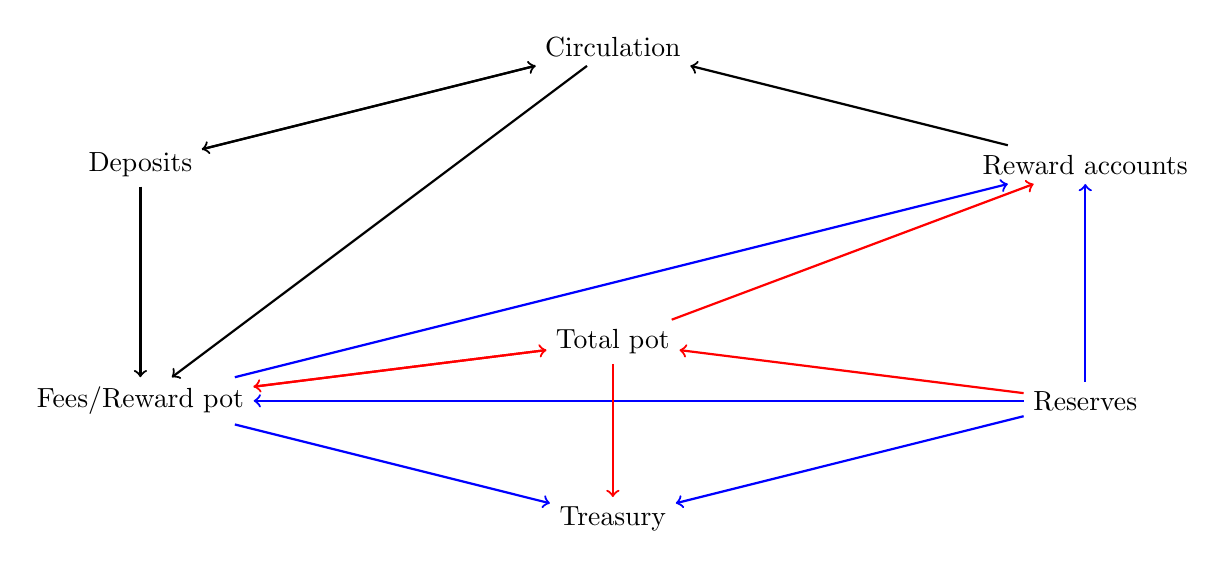
\begin{tikzpicture}
      [ x=30mm, y=30mm
      , direct/.style={black, draw}
      , implied/.style={blue, draw}
      , toTotPot/.style={red, draw}
      ]
    \node (C) at (3,2.5) {Circulation};
    \node (R) at (5, 1) {Reserves};
    \node (D) at (1, 2) {Deposits};
    \node (FR) at (1,1) {Fees/Reward pot};
    \node (RA) at (5, 2) {Reward accounts};
    \node (T) at (3,0.5) {Treasury};

    \draw[->, direct, thick]
    (C) edge (D)
    (C) edge (FR)

    (D) edge (C)
    (D) edge (FR)

    (RA) edge (C);

    \draw[->, implied, thick]
    (FR) edge (T)
    (FR) edge (RA)

    (R) edge (FR)
    (R) edge (T)
    (R) edge (RA);

    \node (TP) at (3, 1.25) {Total pot};

    \draw[->, toTotPot, thick]
    (FR) edge (TP)
    (R) edge (TP)

    (TP) edge (RA)
    (TP) edge (FR)
    (TP) edge (T);

  \end{tikzpicture}
  \end{center}
  \caption{Preservation of Value}
  \label{fig:fund-preservation}
\end{figure}

Figure~\ref{fig:rules:reward} defines the reward transition rule.
The reward transition has no preconditions.

\begin{itemize}
  \item First we calculate $\var{totalPot}$, the total amount of coin avail for rewards this epoch,
    , as described in section 6.4 of \cite{delegation_design}. It consists of four pots:
    \begin{itemize}
      \item The fee pot, containing the transaction fees from the epoch.
      \item The amount of coin in the deposit pot that is no longer needed, due to decay.
      \item The reward pot, which is the left-over rewards from the previous epoch.
      \item Some amount of monetary expansion from the reserves, as determined by the
        $\rho$ protocol parameter.
    \end{itemize}
    Note that the fee pot and the decayed amount are taken from the snapshot taken at the
    epoch boundary.  (See~Figure\ref{fig:rules:snapshot}).
  \item Some proportion of the total pot is moved to the treasury,
    as determined by the $\tau$ protocol parameter. The remaining pot is called the
    $\var{R}$, just as in section 6.5 of \cite{delegation_design}.
  \item The rewards are calculated, using the oldest stake distribution snapshot (the one
    labeled ``go'').
    As given by $\fun{maxPool}$, each pool can receive a maximal amount, determined by its
    performance.  The difference between the maximal amount and the actual amount received is
    moved to the treasury.
  \item The reward pot is now set to $\var{R}$ less the total amount of rewards
    actually paid out and the unrealized rewards given to the treasury.
  \item The moving averages are updated.  Note the averages were already computed on the previous
    epoch boundary, as a part of the stake distribution calculation, and could therefore
    be cached in order to prevent calculating them twice.
  \item The fee pot is reduced by $\var{feeSS}$.
\end{itemize}

Note that fees are not explicitly removed from any account:
the fees come from transactions paying them, and are accounted for whenever
transactions are processed, and the deposit decay value comes from returning
smaller refunds for deposits than were paid upon depositing.

\clearpage

%%
%% Figure - Rewards Rules
%%
\begin{figure}[htb]
  \begin{equation}\label{eq:acnt}
    \inference[Rewards]
    {
      {
      \begin{array}{r@{=}l}
        \left(
          \begin{array}{c}
            \wcard \\
            \wcard \\
            \var{pstate_{go}} \\
            \var{poolsSS} \\
            \var{blocksSS} \\
            \var{feeSS} \\
          \end{array}
        \right) & \var{ss} \\
        \var{expansion} & \floor*{(\fun{rho}~{pp}) \cdot \var{reserves}} \\
        \var{totalPot} & \var{feeSS} + \var{rewardPot} + \var{expansion} \\
        \var{newTreasury} & \floor*{(\fun{tau}~{pp}) \cdot \var{totalPot}} \\
        \var{R} & \var{totalPot} - \var{newTreasury} \\
        \var{rewards'},~\var{unrealized}
          & \reward{pp}{blocksSS}{R}{(\dom{rewards})}{poolsSS}{avgs}{pstake_{go}} \\
        \var{newTreasury'} & \var{newTreasury} + \var{unrealized} \\
        \var{paidRewards} & \left(
                            \sum\limits_{\_\mapsto c\in\var{rewards'}}c
                            \right) + \var{unrealized} \\
        \var{avgs'} & \updateAvgs{pp}{avgs}{blocks}{pooledStake} \\
      \end{array}
      }
    }
    {
      \begin{array}{l}
        \var{pp}\\
        \var{blocks}\\
        \var{ss}\\
      \end{array}
      \vdash
      \left(
        \begin{array}{r}
          \var{treasury} \\
          \var{reserves} \\
          \var{rewardPot} \\
          ~ \\
          \var{stkeys} \\
          \var{rewards} \\
          \var{delegations} \\
          \var{ptrs} \\
          ~ \\
          \var{stpools} \\
          \var{poolParams} \\
          \var{retiring} \\
          \var{avgs} \\
          ~ \\
          \var{utxo} \\
          \var{deposits} \\
          \var{fees} \\
        \end{array}
      \right)
      \trans{reward}{}
      \left(
        \begin{array}{rcl}
          \varUpdate{\var{treasury}} & \varUpdate{+} & \varUpdate{\var{newTreasury'}} \\
          \varUpdate{\var{reserves}} & \varUpdate{-} & \varUpdate{\var{expansion}} \\
          \varUpdate{\var{R}} & \varUpdate{-} & \varUpdate{\var{paidRewards}} \\
          ~ \\
          \var{stkeys} \\
          \varUpdate{\var{rewards}} & \varUpdate{\unionoverridePlus} & \varUpdate{\var{rewards'}} \\
          \var{delegations} \\
          \var{ptrs} \\
          ~ \\
          \var{stpools} \\
          \var{poolParams} \\
          \var{retiring} \\
          \varUpdate{\var{avgs'}} \\
          ~ \\
          \var{utxo} \\
          \var{deposits} \\
          \varUpdate{fees} & \varUpdate{-} & \varUpdate{feeSS} \\
        \end{array}
      \right)
    }
  \end{equation}
  \caption{Rewards inference rules}
  \label{fig:rules:reward}
\end{figure}
